\chapter{Двухчастотное волновое смешение на кубите: случай непрерывных волн}
\label{ch: cwm}
Основные экспериментальные результаты работы заключается в изучении волнового смешения на двухуровневой системе, играющей роль искусственного атома в открытом пространстве. Прежде чем перейти конкретно к выполненному в рамках работы эксперименту --- рассеянию двух почти резонансных микроволн на кубите --- рассмотрим основные принципы волнового смешения в том классическом виде, в котором оно описывается в нелинейной оптике сплошных сред для случая смешивания на ансамблях двухуровневых систем.
\section{Оптическое волновое смешение: случай распределенной среды и слабого пробного сигнала}
Рассматриваемый в имеющейся литературе по нелинейной оптике случай волнового смешения является одним из примеров большого класса нелинейных параметрических процессов --- процессов генерации новых частотных компонент или изменения исходных компонент при распространении света в нелинейной среде. Такие процессы удобно описывать при помощи волнового уравнения, учитывающего нелинейную поляризацию среды $\mathbf{P}^{N\!L}$. В классическом учебнике \cite{boyd2003nonlinear} показано, что данное уравнение можно записать для каждой частотной компоненты поля в виде:
\begin{equation}
\left( \frac{\partial^2}{\partial x^2} + k_n^2\right) \mathbf{E}_n(\mathbf{r}) = -\frac{k_n^2}{\varepsilon\varepsilon_0}\mathbf{P}^{N\!L}_n(\mathbf{r}),
\label{eq: P_NL}
\end{equation}
где роль <<внешнего силы>> играет нелинейная часть электрической поляризации $\mathbf{P}^{N\!L}_n(\mathbf{r}) = \mathbf{P}_n(\mathbf{r}) - \mathbf{P}^{1}_n(\mathbf{r})$. Отметим, что в нелинейную часть могут входить и линейные по электрическому полю слагаемые, но при этом не описывающиеся стандартной формой материальных уравнений. Для ансамбля двухуровневых систем поляризацию можно рассчитать, используя решения динамических уравнений Блоха, рассмотренных в разделе \ref{sec: scatt}. Уравнения Блоха для двухуровневой системы могут быть записаны для заселенности кубита $z = \rho_{11}-\rho_{00}$ и для поляризации кубита $p=\mu_{01}\rho_{10}$ в следующем виде:
\begin{equation}
\systeme{\frac{dp}{dt} = \left(\Delta-i\Gamma_2\right)p -\frac{i}{\hbar}|\mu_{01}|^2Ez,
	\frac{dz}{dt} = -(z-z^{(eq)})\Gamma_1 + \frac{4}{\hbar}\text{Im}(pE^*)},
\label{eq: bloch_p_z}
\end{equation}
где $\Delta = \omega - \omega_{01}$.
В рассматриваемом случае нас интересует поведение двухуровневой системы под действием двух взаимодействующих с ней волн:
\begin{equation}
\tilde{E}(t) = Ee^{-i\omega t} = E_0e^{i\omega t} + E_1e^{i(\omega+\delta) t},
\label{eq: field}
\end{equation}
то есть, под действием волны накачки c произвольной (и возможно, достаточно большой) амплитудой $E_0$, и отстроенной от накачки на величину $\delta$ пробной волны малой амплитуды $E_1 \ll E_0$. Внешнее поле \eqref{eq: field} таково, что решение уравнений \eqref{eq: bloch_p_z} необходимо искать в виде:
\begin{align}
p &= p_0 + p_1 e^{-i\delta t} + p_{-1}e^{i\delta t}, \\
z &= z_0 + z_1 e^{-i\delta t} + z_{-1}e^{i\delta t},
\label{eq: sol_bloch_WM}
\end{align}
предполагая при этом, что $|p_0| \gg |p_1|, |p_{-1}|$~и~$z_0 \gg z_1, z_{-1}$.  При учете только первого порядка малости дополнительных компонент, решение этих уравнений прямолинейно, но достаточно громоздко. Опуская подробности, приведем результат решения \eqref{eq: bloch_p_z} для заселенности на частоте драйва $z_0$, заселенности на пробной частоте $z_1$ и поляризации на пробной частоте $p_{\m}$, и наконец, поляризации $p_{-1}$ на  комбинационной частоте $\omega-\delta = 2\omega - (\omega+\delta)$:
\begin{align}
z_0 &=  - {{1+\Delta^2/\Gamma_2^2} \over {1+ \Delta^2/\Gamma^2_2 + \Omega^2/\Gamma_1\Gamma_2}}, \label{eq: z_0} \\
z_1 &=   - z_0\Omega^2{{E_1} \over {2E_0}} \frac{(\delta-\Delta + i\Gamma_2)(\delta+2i\Gamma_2)}{(\Delta-i\Gamma_2)D(\delta)}, \\
p_1 &=  \frac{|\mu_{01}|^2z_0E_1}{\hbar D(\delta)}\left[\left(\delta + i\Gamma_1\right)\left(\delta-\Delta+i\Gamma_2\right)-\frac{\delta\Omega^2}{2(\Delta-i\Gamma_2)}\right], \label{eq: p1}\\
p_{\m} &=  2 z_0 \frac{|\mu_{01}|^4E_0^2E_1^*}{\hbar^3 D^*(\delta)}\frac{(\delta-\Delta-i\Gamma_2)(-\delta+2i\Gamma_2)}
{(\Delta + i\Gamma_2)(\Delta-\delta+i\Gamma_2)}. \label{eq: p-1}
\end{align}
В записи этих выражений использовано обозначение:
\begin{equation}
D(\delta) = \left( \delta + i\Gamma_1\right) \left(\delta-\Delta +i\Gamma_2\right) \left(\delta+\Delta +i\Gamma_2\right)-\Omega^2\left(\delta+i\Gamma_2\right)
\end{equation}
В решении \eqref{eq: z_0}-\eqref{eq: p-1} нас интересуют поляризации \eqref{eq: p1} и \eqref{eq: p-1}, которые определяют эффективную линейную восприимчивость и восприимчивость третьего порядка:
\begin{equation}
\begin{aligned}
\chi^{(1)}_{\text{eff}}(\omega+\delta) &=  \frac{p_1}{\varepsilon_0 E_1}, \\
\chi^{(3)}_{\text{eff}}(\omega-\delta = 2\omega-(\omega+\delta)) &=  \frac{p_{\m}}{3\varepsilon_0 E^2_0 E_1^*}.
\label{eq: P_eff}
\end{aligned}
\end{equation}
При расчете полных поляризаций $P(\omega+\delta)$ и $P(\omega-\delta)$ необходимо учитывать отклик среды на поле, возникающее на комбинационной частоте, поэтому каждая из поляризаций имеет как линейный, так и кубический вклад:
\begin{equation}
\begin{aligned}
P(\omega+\delta) &=  \varepsilon_0 \chi^{(1)}_{\text{eff}}(\omega+\delta) E_1 +  3\varepsilon_0 E^2_0 E_{\m}^*\chi^{(3)}_{\text{eff}}(\omega+\delta = 2\omega-(\omega-\delta)), \\
P(\omega-\delta) &=  \varepsilon_0 \chi^{(1)}_{\text{eff}}(\omega-\delta) E_{\m} +  3\varepsilon_0 E^2_0 E_1^*\chi^{(3)}_{\text{eff}}(\omega-\delta = 2\omega-(\omega+\delta)).
\label{eq: P_total}
\end{aligned}
\end{equation}
Выражения для поляризаций можно подставить в волновое уравнение \eqref{eq: P_NL} и искать решение этого уравнения, представляя каждую частотную компоненту поля $E_n$ через комплексные амплитуды:
\begin{equation}
E_n = A_n e^{-i(\omega_nt - k_nx)} + \text{c.c.},
\label{eq: E_complex}
\end{equation}
%где мы ввели комплексную амплитуду $A_n$, не меняющуюся во времени.  Для простоты будем считать, что среда обладает только нелинейностью третьего порядка, и среди всех параметрических процессов этого порядка нас интересует компоненты, возникающие за счет вклада в поляризацию на частоте $\omega_{-1} = 2\omega_0-\omega_1$ следующего вида:
%\begin{equation}
%\tilde{P}^{N\!L} = {P}_{-1} e^{-i(2\omega_1-\omega_0)t} + \text{c.c.}= 3\varepsilon_0\chi^{(3)}E_0^2E_1^*e^{-i(2\omega_1-\omega_0)t} + \text{c.c.}.
%\end{equation} 
%После подстановки в это уравнение выражений \eqref{eq: E_complex} для компоненты на боковой частоте имеем:
%\begin{equation}
%P_{-1} = 3\varepsilon_0\chi^{(3)}A_0^2A_1^*e^{i(2k_0-k_1)z}.
%\end{equation}
%Имея выражение для поляризации на нужной частоте, можем записать \eqref{eq: P_NL} для комплексной амплитуды поля, возникшего за счет смешения:
%\begin{equation}
%ку \left[ \frac{\partial^2}{\partial z^2} A_{\m} - 2ik_{\m}\frac{\partial}{\partial z}A_{\m}\right] + \text{ c.c.} = 3\frac{\chi^{(3)}k^2_{\m}}{\varepsilon} A_0^2A_1^* e^{i(2k_0-k_1-k_{\m})z} + \text{ c.c.}
%\end{equation}
%Считая, что амплитуда медленно меняется во времени, можно пренебречь слагаемым $\partial^2A_{\m}/\partial z^2$. Далее, поскольку эффект связывает слабые поля на частотах $\omega_1$ и $\omega_{\m}$, то необходимо проделать всю процедуру для поля с амплитудой $A_1$. 
В итоге получается система обыкновенных дифференциальных уравнений для комплексных амплитуд:
\begin{equation}
\systeme{
\frac{\partial A_1}{\partial x} = -\alpha_1 A_1 + \kappa_1A^*_{\m} e^{i\Delta k x}\text{,},
\frac{\partial A_{\m}}{\partial x} = -\alpha_{\m} A_{\m} + \kappa_{\m}A^*_1 e^{i\Delta k x}.
\label{eq: compl_ampl}}
\end{equation}
где параметры $\alpha_{\pm1}\propto\text{Im}\left(\chi^{(1)}_{\text{eff}}(\omega\pm\delta)\right)$ характеризуют потери, а параметр $ \kappa_{\pm1}\propto\chi^{(3)}_{\text{eff}}(\omega\pm\delta)$ определяют величину взаимодействия мод через нелинейную среду. Расхождение волновых векторов $\Delta \textbf{k} = |2\textbf{k}_0 - \textbf{k}_1 - \textbf{k}_{-1} |$ обусловлено дисперсией материала, и зависит от геометрии пучков. Ясно, что даже если $A_{-1}(0) = 0$, в общем случае уравнения для амплитуд связаны, и поэтому при распространении волны вдоль материала $A_{-1}(x) \ne 0$ --- происходит перекачка энергии в поле на комбинационной частоте, что и соответствует волновому смешению. 
Решения уравнений \eqref{eq: compl_ampl} подробно исследовались в работе \cite[]{Boyd_WM_81}, в частности, показано, что при некоторых параметрах происходит усиление пробного сигнала при $\delta \approx 0$ и $\delta \approx \Omega$.

Кратко изложив формализм, позволяющий получить волновое смешение в нелинейной среде, необходимо отметить, что его прямое применение для изучения смешивания на кубите в линии достаточно затруднено. Во-первых, основные результаты выведены в предположении, что амплитуда пробной волны значительно меньше амплитуды накачки. Во-вторых, дисперсия в копланарной линии на частотах кубита отсуствует: $\omega \propto k$. Также геометрия рассеяния одномерна, и поэтому с достаточной точностью выполнено условие фазового синхронизма $\Delta k =0$, справедливость которого особенно трудно обеспечить для оптики видимого диапазона, где направления различных лазерных пучков могут быть различны. Добавим, что нас мало интересует координатная зависимость амплитуд, потому как кубит в волноводе представляет собой точечный нелинейный объект, в отличие от типичных нелинейных сред (оптоволокно, кристаллы), и нет цели синхронизовать нелинейный отклик различных пространственных частей протяженной среды. 

Эксперименты, выполняемые в рамках диссертации, далеки от случая слабой пробной волны и относятся к ситуации, когда на двухуровневый атом действует два сильных поля с Раби частотами $\Omega_1, \Omega_2$. Эта накачка известна под термином \textit{бихроматическая накачка}, и в дальнейшем подразделе мы опишем известные результаты для двухуровневой системы под действием накачки данного типа. 

\section{Спектр резонансной флуоресценции в случае бихроматической накачки}

Случай бихроматической накачки на двух различных частотах представляет собой логичное обобщение стандартной задачи рассеяния монохроматической волны на атоме. Для того, чтобы раскрыть механизм рассеяния света на атоме, обычно прибегают к расчету и измерению спектра рассеянного света.

Спектр резонансной флуоресценции в целом является достаточно информативной характеристикой квантовой системы: его вид позволяет выявить структуру состояний квантовой системы, возникшую под действием поля. Говорят, что система <<одевается>> полем, а гибридизованные собственные состояния называются \textit{одетыми} состояниями. В наиболее простом случае двухуровневой системы, взаимодействующей с сильным монохроматическим сигналом, спектр представляется в виде триплета Моллоу, детально рассмотренного в разделах \ref{sec: scatt} и \ref{sec: Triplet_meas}. Однако, оказалось что при возбуждении кубита бихроматической накачкой происходят кардинальные качественные изменения в общем виде спектра. Кратко рассмотрим известные результаты для полного спектра излучения под действием бихроматической накачки. 


В разделе \ref{sec: scatt} спектр резонансной флуоресценции был посчитан при помощи решения уравнений динамики кубита и квантовой регрессионной теоремы. Однако, приближенный вид спектра во многих случаях можно определить с использованием формализма одетых состояний, впервые предложенного Клодом Коэном-Таннуджи в статье \cite{cohen1977dressed} и также изложенного в книге \cite{cohen1998atom}. Алгоритм действий состоит в следующем:
\begin{enumerate}
	\item \label{levs} Записывается гамильтониан атома и одномодовый гамильтониан поля и находятся невозмущенные уровни этой системы. В простейшем случае двухуровнего атома и одной моды поля собственные состояния невзаимодействующего атома и поля представляются в виде $\ket{g, N},\!\ket{e, N-1},\!\ket{f, N-2},$\ldots, где первое квантовое число обозначает состояния атома, а второе --- число фотонов в полевой моде. 
	\item В исходной системе уровней, определенной в п.~\ref{levs}, можно выделить два типа дипольно разрешенных переходов. Переходы первого типа происходят между состояниями $\ket{e,N-1} \leftrightarrow \ket{g,N}$ соответствуют когерентной передаче возбуждений из полевой моды в атом. Поскольку состояние поля предполагается когерентным с $|\alpha| \gg 1$, то вклад в когерентное излучение будет определяться всеми фоковскими состояниями поля, попадающими в полосу с  дисперсией $\Delta N$, при этом $1 \ll \Delta N \ll |\alpha^2|$. Переходы второго типа $\ket{g, N} \leftrightarrow \ket{e, N} $ происходят по причине спонтанного излучения фотонов в другие моды и поэтому определяют спектр неэластично рассеянного света. 
	\item К гамильтониану добавляется член, выражающий взаимодействие поля и атома. Взаимодействие снимает вырождение уровней с одинаковым числом возбуждений в резонансном случае, и диагонализация вырожденных подпространств позволяет найти новые собственные состояния <<одетого>> полем атома.
	\item \label{bohr}Новые собственные векторы одетого полем атома в некоторой пропорции включают в себя векторы $\ket{g, N}$ и $\ket{e, N}$, поэтому спонтанная эмиссия происходит между каждой парой уровней одетого базиса, где верхний одетый уровень содержит ненулевой вклад от уровня $\ket{e, N}$, а нижний одетый уровень содержит вклад от уровня $\ket{g,N}$. Боровские частоты этих разрешенных переходов немедленно дают частоты пиков, наблюдающихся в спектре неэластичного рассеяния.
	\item Интенсивности и ширины пиков на частотах, определенных в п.~\ref{bohr}, могут быть определены после решения квантового основного уравнения для одетого атома. Необходимо отметить, что для получения корректных значений для ширин и высот пиков необходимо точно учесть каскадные процессы спонтанной эмиссии, при которых атом спускается по лестнице уровней посредством спонтанного распада между подсистемами уровней с различным значением $N$.
\end{enumerate}
Данный метод дает количественно правильные результаты для двухуровневого атома и монохроматического поля, но при этом легко обобщается на случай бихроматического поля. 

Рассмотрим симметричный случай бихроматической накачки двумя волнами, частоты Раби которых равны: $\Omega_+=\Omega_-=\Omega$, которые отстроены от атомного перехода на $\pm \delta$. Метод приблизительного расчета спектра на основе одетых состояний был применен в работах \cite{Freedhoff_resonance}, где была вычислена только неэластичная часть излучения, и \cite{Agarwal:91}, где показан полный спектр резонансной флуоресценции. 

Вначале опишем спектр неэластичного излучения. Он состоит из большого количества эквидистантных пиков, положение которых не зависит от $\Omega$, но общее количество становится больше по мере увеличения амплитуды драйва. Частоты этих пиков определяются соотношением $\omega_q \pm n\delta$, а их  относительная высота и ширина сильно зависит от $\Omega$. Пики разделяются на четные и нечетные, в зависимости от четности $n$, а ширины пиков описываются формулами:
\begin{equation}
\Gamma_{{\substack{\text{even}\\ \text{odd} }}} = \frac{1}{4}\Gamma_1\left[3\mp J_0\left(-\frac{8\Omega}{\delta}\right)\right]
\end{equation}
Расширение этого результата на случай произвольных отстроек и частот Раби проведено в \cite{Ficek_resonance}, также отметим экспериментальное исследование \cite{Zhu_experiment}, которое и вызвало повышенное внимание 
теоретиков к этой задаче. 
Теперь обратимся к эластично рассеянному свету. В комментарии \cite{Comment_resonance} отмечено, что частоты эластичного рассеяния определяются комбинационным правилом $\omega_q \pm (2k+1)\delta$, что совпадает с четными частотами неэластичного рассеяния, хотя и не приводится расчетов полной интенсивности отдельных пиков.
Как показано в \cite{Agarwal:91}, эластичный спектр представляет собой набор  когерентных пиков с очень узкой спектральной шириной, которая определяется аппаратной шириной спектра исходного монохроматического поля. В целом, эластичный спектр может быть рассчитан численно при помощи решения Блоховских уравнений для корреляторов спина. Опишем в общих чертах ход рассуждений, используемый при получении этих результатов. 

Согласно квантовой регресионной теореме, динамика коррелляторов вида
\begin{equation}\label{eq: corrs_dyn}
\begin{split}
\Phi_1(t+\tau, t) &= \braket{\sigma_+(t+\tau)\sigma_-(t)} -  \braket{\sigma_+(t+\tau)}\braket{\sigma_-(t)},\\
\Phi_2(t+\tau, t) &= \braket{\sigma_-(t+\tau)\sigma_-(t)} -  \braket{\sigma_-(t+\tau)}\braket{\sigma_-(t)},\\
\Phi_3(t+\tau, t) &= \braket{\sigma_z(t+\tau)\sigma_-(t)} -  \braket{\sigma_z(t+\tau)}\braket{\sigma_-(t)}\\
\end{split}
\end{equation}
описывается однородной частью блоховских уравнений, которые для случая бихроматической накачки на частотах $\omega_\pm = \omega_q \pm \delta$, имеют следующий вид:
\begin{equation}\label{eq: bloch_corr}
\dot{\mathbf{\Phi}} = \left[\begin{matrix}- \Gamma_2 & 0 & - 2\Omega \cos{\left(\delta\omega t \right)}\\0 & - \Gamma_2 & - 2i \Omega \cos{\left(\delta\omega t \right)}\\ \Omega \cos{\left(\delta\omega t \right)} & -  i \Omega \cos{\left(\delta\omega t \right)} & - \Gamma_1
\end{matrix}\right]\mathbf{\Phi}.
\end{equation}
Точка в этом уравнении обозначает производную по $\tau$.
Для поиска решения можно разложить вектор коррелляций в сумму медленно меняющихся компонент:
\begin{equation}\label{eq: floquet}
\mathbf{\Phi} = \sum_{l=-\infty}^{\infty}\mathbf{\Phi}^{(l)}e^{-i(2l+1)\delta\omega (t+\tau),}
\end{equation}
а затем представить каждую компоненту $\mathbf{\Phi}^{(l)}$ через преобразование Лапласа для переменной $z=i(\omega-\omega_q)$. При этом получаются рекурсивные соотношения специального вида:
\begin{equation}\label{eq: corr_rec}
A_l\Phi^{(l)}_3+B_l\Phi^{(l-1)}_3 + C_l\Phi_3 ^{(l+1)} = D_l,
\end{equation}
где константы $A_l-D_l$ зависят от $z$ как от переменной, от частоты Раби, констант релаксации и дефазировки как от параметров, а также от значений коррелляторов в момент $\tau=0$. Последние, в свою очередь, однозначно определяются средними значениями компонент блоховского вектора:
\begin{equation}
\begin{split}
\Phi_1^{(l)}(t=0) &= \exp(il\delta\omega t)\left(\frac{1}{2}+\frac{1}{2}\!\braket{\sigma_z(t)} - \braket{\sigma_-(t)}\!\braket{\sigma_+(t)}\right) \\
\Phi_2^{(l)}(t=0) &= -\exp(il\delta\omega t)\braket{\sigma_-(t)}^2 \\
\Phi_3^{(l)}(t=0) &= -\exp(il\delta\omega t)\braket{\sigma_-(t)}\left(1+\braket{\sigma_z(t)}\right) \\
\end{split}
\end{equation}
Эластичная часть спектра $S_{el}(\omega)$ определяется как фурье-образ корреллятора $\braket{\sigma_+(t+\tau)}\braket{\sigma_-(t)}$. Для нахождения этого спектра удобно записать для компонент спина разложение по периодическим компонентам, идентичные \eqref{eq: floquet}:
\begin{equation}
\braket{\vec{\sigma}}  = \sum_{l=-\infty}^{\infty}\braket{\vec{\sigma}^{(l)}}\exp(-i(2l+1)\delta\omega t)
\end{equation} и рекуррентные соотношения по типу \eqref{eq: corr_rec}. При этом получаем
\begin{equation}
S_{el}(\omega) = \sum_{l=-\infty}^{\infty}\delta(\omega-\omega_q+(2l+1)\delta\omega)|\!\braket{\sigma_-^{(l)}}\!|^2
\end{equation}
В работе \cite{Ryuten} рекурсивные соотношения для различных компонент спина были решены с помощью метода бесконечных дробей. При этом для случая равных и симметрично расположенных относительно кубита компонент внешнего поля, а также при достаточно медленной релаксации, можно получить следующее выражение:
\begin{equation}
\braket{\sigma_-^{(l)}} = \frac{J_0(x)J_{2l+1}(x)}{1+\Gamma_2/\Gamma_1+ (1-\Gamma_2/\Gamma_1)J_0(2x)},
\end{equation}
где $x=2\Omega/\delta\omega$.  Тогда интенсивность излучения на частоте $\omega_q + (2l-1)\delta\omega$ может быть рассчитана в виде $I_{2l+1} = |\braket{\sigma_-^{(l)}}|^2 + |\braket{\sigma_-^{(-l)}}|^2$. График интенсивности для различных $l$ приведен на Рис. \ref{fig: zeros}, особенностью является нетривиальное распределение нулей компонент, которое определяется функциями Бесселя. 
\begin{figure}[h]
	\centering
	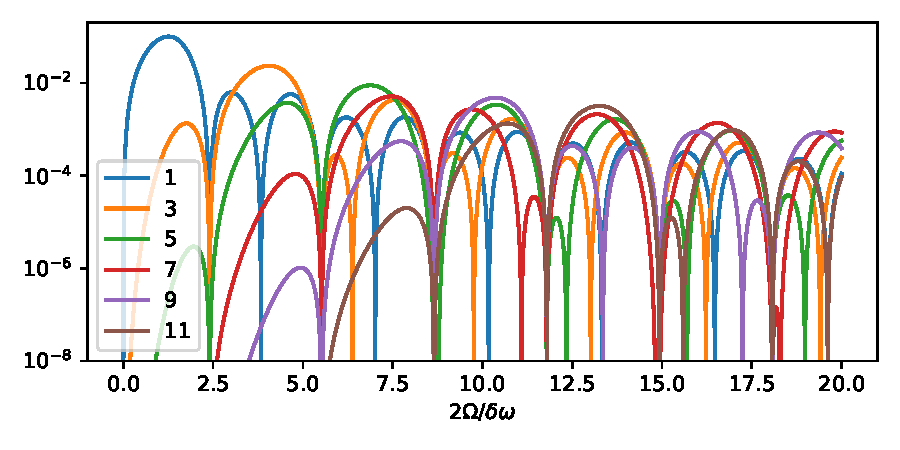
\includegraphics[width=0.95\textwidth]{zeros}
	\caption[Зависимость компонент эластичного рассеяния $I^{2l+1}(2\Omega/\delta\omega)$ для бихроматической накачки.]{Зависимость интенсивности компоненты эластичного рассеяния $I^{2l+1}(2\Omega/\delta\omega)$ для случая бихроматической накачки.}
	\label{fig: zeros}
\end{figure}
Подобную картину можно получить и при помощи рассмотрения одетого атома, однако в вышеупомянутых работах не приводится конкретных результатов для эластичного спектра, полученных на основе этого подхода. 

Мы рассмотрели известные теоретические и экспериментальные результаты для рассеяния бихроматического света на двухуровневой системе. По результатам рассмотрения можно отметить, что в данной работе впервые осуществляется систематическое экспериментальное исследование эластичного рассеяния: ранее в рамках традиционной оптики данный аспект изучался только теоретически, а известные экспериментальные работы \cite{Chakmakjian:88,Zhu_experiment} имеют дело только с неэластично рассеяным излучением. При этом, с точки зрения теории отдельно не рассматривался режим, в котором отстройка компонент драйва от резонанса кубита пренебрежимо мала по сравнению с излучательной шириной кубита.  Рассмотрев известные результаты, мы переходим к выполнявшимся в рамках работы экспериментам по рассеянию бихроматического света на одиночном сверхпроводящем кубите.
\section{Спектр эластичного рассеяния в случае $\delta \ll \Gamma_1$}
Исследование нелинейного рассеяния на одиночном кубите резонно начать с приложения к кубиту двух непрерывных волн. В рамках микроволновой техники наиболее просто использовать в качестве драйва выходные сигналы фазостабильных СВЧ-генераторов. В лаборатории искусственных квантовых систем для этого используются модели Keysight MXG N8257B и EXG N5283. Эти модели обеспечивают перестройку частоты в пределах до 20 ГГц, относительную аппаратную ширину линии порядка $10^{-11}$ и могут быть частотно синхронизированы друг с другом с такой же точностью. Кроме того, в качестве источника может использоваться и выход ВАЦ Keysight PNA-L, обладающий схожими характеристиками, но имеющий в качестве недостатка слабое подавление гармоник исходного синусоидального сигнала --- впрочем, этот эффект не является критическим для использования в обсуждаемом эксперименте. Для того, чтобы завести два непрерывных сигнала с различных источников в единый волновод, достаточно использовать СВЧ-делитель (splitter или power combiner) перед входом сигнала в криостат, объединенный выход которого направляется на вход криостата. Включение одного из источников позволяет произвести стандартные измерения однотоновой спектроскопии, зависимости линии кубита от мощности и резонансной флуоресценции, результаты которых рассматривались в разделах \ref{sec: spectr}-\ref{sec: Triplet_meas}. Нас же интересует спектр рассеянного на кубите сигнала, состоящего из двух компонент от разных источников.

Для решения поставленной задачи по измерению спектра эластичного рассеяния выход волновода с кубитом подключается к спектральному анализатору.  Зная естественную ширину его линии $\Gamma_1$, мы выбираем центральную частоту драйва $\omega_d$ близкую к частоте $\omega_q$ и устанавливаем на СВЧ-генераторах частоты $\omega_\pm = \omega_d \pm \delta\omega$, где величина отстройки $\delta\omega$ много меньше $\Gamma_1$, поскольку мы хотим остаться в резонансном приближении. Установив частоты, мы выравниваем мощности сигналов и начинаем синхронно увеличивать Раби амплитуды драйвов $\Omega_+ = \Omega_- = \Omega$, снимая получающийся спектр. При этом полоса входного фильтра спектрального анализатора может быть выбрана на уровне нескольких Гц, поскольку мы хотим максимально убрать шум и увидеть только эластичную часть сигнала, спектральная ширина которой очень мала.
\begin{figure}[thb]
	\centering
	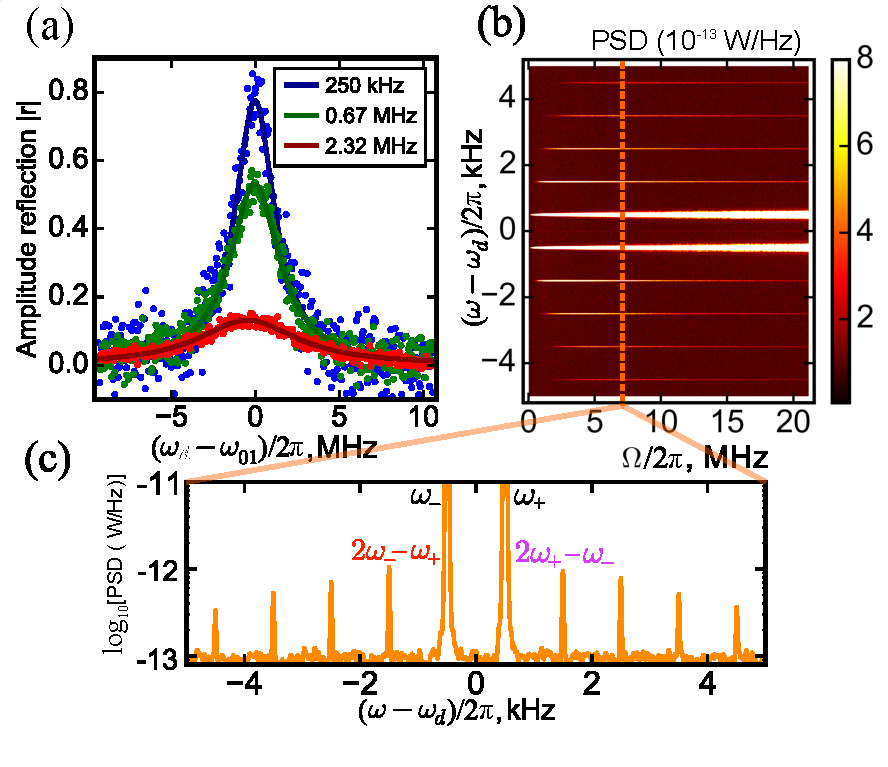
\includegraphics[width=0.85\textwidth]{Fig_2_fixed_PRA_forThesis.pdf}
	\caption[Волновое смешение: появление дополнительных компонент эластично рассеянного сигнала]{(a) Коэффициент прохождения $S_{21}$ одиночной резонансной волны на кубите в зависимости от отстройки $\Delta\omega = \omega_d-\omega_q$, при различных значениях частоты Раби. Параметры кубита $\Gamma_1/2\pi = 2.2$~МГц, $\Gamma_2 = \Gamma_1/2$. (b) Цветовой график спектров рассения двух волн на частотах $\omega_{\pm}$ в зависимости от частоты Раби для $\delta\omega = 1$ kHz. (c) Пример спектра при $\Omega/2\pi=7$~МГц. }
	\label{fig: CWM}
\end{figure}
Результаты измерений приведены на Рис.~\ref{fig: CWM}. Качественное поведение спектра по мере увеличения $\Omega$ хорошо проиллюстрировано на Рис.~\ref{fig: CWM}b). При увеличении Раби-частоты от нуля до нескольких единиц $\Gamma_1$ появляется большое количество эластичных пиков, частоты которых равны $\omega_{\pm(2p+1)} = (p+1)\omega_\pm-p\omega_\mp$ и интенсивности которых достигают своего максимума при определенных значениях $\Omega$, а в дальнейшем плавно спадают, см.  Рис.~\ref{fig: CWM}с). Дополнительно были измерены зависимости спектра смешения при постоянной амплитуде волны на отрицательно смещенной частоте при увеличении амплитуды волны на положительно смещенной частоте, начиная от очень низкой амплитуды $\Omega_+ \ll \Gamma_1$ и заканчивая высокой амплитудой $\Omega \gg \Gamma_1$. Результаты этих измерений изображены на см. Рис.~\ref{fig: cw_power_sweep}. 

Таким образом, экспериментально показан эффект волнового смешения непрерывных волн на одиночной нелинейности в волноводе. В данном измерении на пути сигнала не имеется никаких нелинейных элементов, которые мы могли бы вызвать подобное рассеяние. В качестве подтверждения, аналогичные измерения были проведены при большой отстройке кубита $\Delta\omega = \omega_q - \omega_d \gg \Gamma_1 $, и в этом режиме не было обнаружено дополнительных спектральных компонент. Таким образом, можно считать доказанным факт наблюдения волнового смешения на одиночном сверхпроводящем атоме в волноводе.  
\begin{figure}
	\centering
	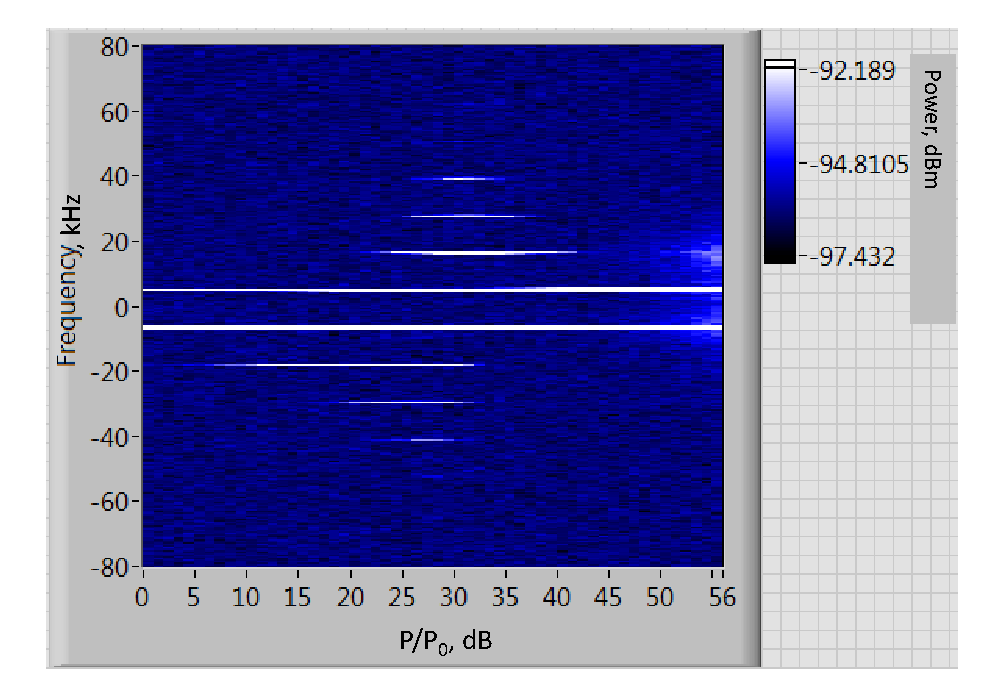
\includegraphics[width=0.8\textwidth]{cwm_power_sweep.pdf}
	\caption[Зависимость спектра смешения от амплитуды волны $\Omega_+$ при фиксированной амплитуде волны $\Omega_-$. ]{Зависимость спектра смешения от амплитуды волны $\Omega_+$ при фиксированной амплитуде волны $\Omega_-$.}
	\label{fig: cw_power_sweep}
\end{figure}
В режиме непрерывной бихроматической накачки интерес представляет снятие зависимости компонент напряжения, отвечающих дополнительным спектральным линиям, от частоты Раби $\Omega$, и сопоставление  полученного результата с аналитическим расчетом. Более того, поскольку имеется возможность менять $\Omega_+$ и $\Omega_-$ независимо, представляет интерес показать, как меняется в этом случае вид спектра эластичного рассеяния. Как будет показано в следующем разделе, для расчета спектра в режиме $\delta\omega \ll \Gamma_1$, в котором проводятся практически все излагаемые ниже измерения, можно воспользоватся аналитическим выражением \eqref{eq: refl} для поля, излучаемого кубитом в стационарном режиме в случае монохроматического драйва и получить выражения для амплитуд напряжений и мощностей боковых компонент поля $\Omega_{\pm(2p+1)}$, выраженных в единицах частоты Раби. Физический смысл этих компонент следует из соотношения $\hbar\Omega_{\pm(2p+1)} = \mu V_{\pm{2p+1}}$. Также мы проведем сравнение полученных формул с экепериментальными данными и обсудим потенциальные применения данного эффекта.

\section{Аналитическое выражение для амплитуд боковых гармоник в приближении малой отстройки}
\label{sec: anal_sol}

Для расчета амплитуд дополнительных гармоник, появляющихся в результате волнового смешения, запишем гамильтониан для двухуровневой системы, дипольно связанной с континуумом мод волновода, в котором распространяется вышеупомянутое бихроматическое поле. Гамильтониан имеет следующий вид:
\begin{equation}	
H = -\frac{\hbar \omega_{01}}{2}\sigma_z -\hbar \Omega_- \sigma_x \cos(\omega_d t - \delta\omega t) -\hbar \Omega_+ \sigma_x \cos(\omega_d t + \delta\omega t),	
\end{equation} 
где $\Omega_+$ и $\Omega_-$ определены выше. Для начала мы рассчитаем стационарное решение основного квантового уравнения для данного гамильтониана в приближении вращающейся волны. Член  $\delta\omega t$, стоящий под знаком косинуса, будет рассматриваться здесь как медленно меняющаяся во времени фаза, потому что  $\delta\omega t \ll 1$ на масштабе времени когерентности $t \sim \Gamma_2^{-1}$ кубита. Аналитическое решение для среднего значения оператора понижения для атома имеет вид:  
\begin{equation}
\langle \sigma^-\rangle = -\frac{\sin\theta}{\Lambda} \frac{\Omega_- e^{-i\delta\omega t} + \Omega_+ e^{i \delta\omega t}}{1 + \sin\theta\cos{2\delta\omega t}}. 
\label{exp_value}
\end{equation}
%Here we introduce the following notations: $\frac{1}{\Lambda} = \frac{\Gamma_1 \lambda}{2D}$, $\beta = \frac{2\Gamma_2 \Omega_- \Omega_+}{D}$, where $\lambda = \Delta \omega - i\Gamma_2$, $D = \Gamma_1 |\lambda|^2 + \Gamma_2(\Omega_-^2 + \Omega_+^2)$.
Здесь введены следующие обозначения: $\theta = \arcsin\Big(\frac{2\Gamma_2 \Omega_- \Omega_+}{\Gamma_1 |\lambda|^2 + \Gamma_2(\Omega_-^2 + \Omega_+^2)}\Big)$, $\Lambda^{-1} = \frac{\lambda\Gamma_1}{4\Gamma_2 \Omega_-\Omega_+}$, $\lambda = \Gamma_2 + i\Delta\omega$.
%\begin{align*}
%A = \frac{\Gamma_1 \lambda}{2D}, 
%\beta & = \frac{2\Gamma_2 \Omega_- \Omega_+}{D}, \lambda = \Delta \omega - i\Gamma_2, \\
%D & = \Gamma_1 |\lambda|^2 + \Gamma_2(\Omega_-^2 + \Omega_+^2).
%\end{align*} 
Знаменатель уравнения~\eqref{exp_value} можно переписать согласно соотношению  
\begin{equation}
%\langle \sigma^-\rangle = \frac{\Omega_- e^{-i\delta\omega t} + \Omega_+ e^{i \delta\omega t}}{\alpha \Lambda} \sum_{p=-\infty}^{\infty}y^{|p|} e^{i 2 p \delta\omega t},
\frac{1}{1+\frac{1}{2}\sin\theta(z + z^{-1})} = \frac{1}{\cos{\theta}}\Big(\frac{1}{1- yz} + \frac{1}{1- yz^{-1}}-1\Big), 
%\frac{1}{\cos{\theta}}\sum_{p=-\infty}^{\infty}y^{|p|} e^{i 2 p \delta\omega t},
\label{exp_value2}
\end{equation}
где %$\beta = \frac{y}{1+y^2}$ and $z = e^{2i\delta\omega t} $ 
$z = e^{2i\delta\omega t}$ и $y = -\tan{\frac{\theta}{2}}$. Правая часть уравнения \eqref{exp_value2} раскладывается в степенной ряд по $z$ и мы получаем:
\begin{equation}
%\langle \sigma^-\rangle = \frac{\Omega_- e^{-i\delta\omega t} + \Omega_+ e^{i \delta\omega t}}{\alpha \Lambda} \sum_{p=-\infty}^{\infty}y^{|p|} e^{i 2 p \delta\omega t},
\langle\sigma^-\rangle = -\frac{\Omega_- e^{-i\delta\omega t} + \Omega_+ e^{i \delta\omega t}}{\Lambda}\tan\theta \sum_{p=-\infty}^{\infty}y^{|p|} e^{i 2 p \delta\omega t}.
\label{exp_value3}
\end{equation}
Учитывая, что  $\hbar V_{sc} = -i\Gamma_1\!\braket{\sigma_-}\!/\mu$ и преобразуя сумму к неотрицательным $p$, мы получаем:
\begin{equation}
V^{sc} =  
-\frac{\hbar\Gamma_1\tan\theta}{\mu\Lambda}\sum_{p=0}^{\infty}y^p\Big[ (\Omega_- + y \Omega_+ ) e^{-i(2p+1)\delta\omega t}
+ (y \Omega_- + \Omega_+) e^{i(2p+1)\delta\omega t}\Big].
\label{an_eq}
\end{equation}
Учитывая соотношения $V_\pm \mu = \hbar\Omega_\pm$, мы можем записать результат для Раби-амплитуд дополнительных спектральных компонент, появившихся в результате рассеяния на атоме: 
\begin{equation}
%|\Omega_{\pm(2p+1)}^{sc}|^2 =\left[\frac{\Gamma_1 A}{\alpha} y^{p}(\Omega_{\mp}+y\Omega_{\pm})\right]^2,
\Omega_{\pm(2p+1)}^{sc} =\frac{(-1)^p\Gamma_1\tan\theta\tan^p\frac{\theta}{2}}{\Lambda} (\Omega_{\mp}\tan\frac{\theta}{2} - \Omega_{\pm}),
\label{intensities}
\end{equation} 
которое можно проверить, измеряя интенсивности компонент в эксперименте.

\begin{figure}[thb]
	\centering
	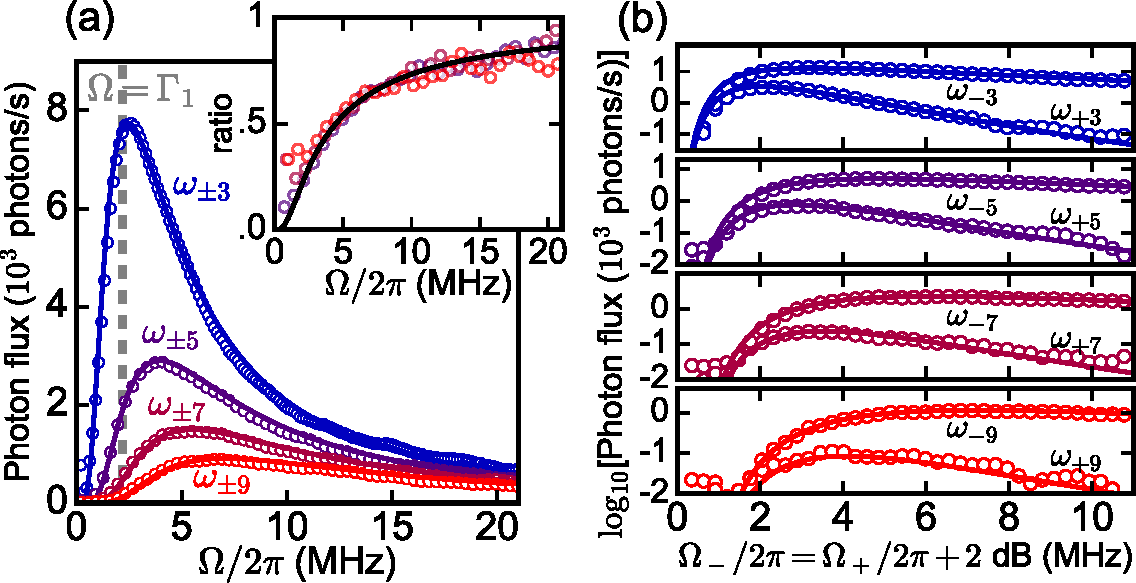
\includegraphics[width=0.9\textwidth]{Fig3_PRA_proofs3.pdf}
	\caption[Эластичные компоненты: сравнение аналитического расчета и экспериментальных результатов ]{(a) Боковые спектральные компоненты эластично рассеянного излучения, выраженные в единицах потока фотонов. Экспериментальные данные получены для $\delta\omega/2\pi=5$~кГц сравниваются с результатом в соответствии с  \eqref{intensities} (сплошные линии) с параметрами $\Gamma_1/2\pi = 2.2$~МГц, $\Gamma_2/2\pi=1.1$~МГц, $\Delta\omega/2\pi=0$, $\Omega_+=\Omega_- =\Omega$ и $p=1,2,3,4$ для каждой из кривых, соотвественно. На вставке приведены отношения потоков для последовательных порядков $2p+1$ и $2p+3$ для $p=1,2,3$. Черная линия представляет прямой расчет отношений согласно \eqref{intensities}. (б) Компоненты волнового смешения при ассимметричном драйве: $\Omega_-$~ на 2 дБ превышает $\Omega_+ $. Поток фотонов в компонентах с отрицательной стороны в несколько раз превышает поток в соответствующих положительных компонентах. Это свидетельствует о высокой чувствительности компонент волнового смешения к неравенству амплитуд сигналов бихроматической накачки.}
	\label{Peaks_WM_with_fit}
\end{figure}

На Рис.~\ref{Peaks_WM_with_fit} проводились измерения интенсивностей спектральных компонент в зависимости от $\Omega_-, \Omega_+$, и результаты этих измерений сравнивались с выражением \eqref{intensities} без применения подгоночных параметров. Рис.~\ref{Peaks_WM_with_fit}(a) представляет потоки фотонов в компонентах для  $1< p < 4$ (вплоть до 9-фотонных процессов) в случае $\Omega_+\!=\!\Omega_-\!=\!\Omega$ как функцию $\Omega$: правые и левые боковые пики в этом случае имеют равные амплитуды. С увеличением $\Omega$, амплитуды боковых пиков достигают максимума и потом уменьшаются, причем по мере увеличения $p$ максимум компоненты соотвествующего порядка достигается при большем значении $\Omega$. Это можно интерпретировать, считая, что порядок компоненты $2p + 1$ соответствует числу взаимодействующих на кубите фотонов из исходных сигналов на частотах $\omega_+, \omega_-$. Скорость испускания и поглощения фотонов определяется частотой Раби, а характеристическое время взаимодействия с кубитом определяется его когерентностью $\tau \sim \Gamma_2$. Поэтому, для эффективного поглощения или излучения фотонов в боковой пик порядка $\pm(2p+1)$ необходимо выполнить условие
\begin{equation}
2\Omega\cdot \tau \approx 2p+1,
\end{equation}
откуда получаем качественную оценку $\Omega_{max} \approx \Gamma_1(2p+1)/4$. Анализируя выражение \eqref{intensities} на предмет экстремума, получаем точные значения максимумов $\Omega_{max} = \sqrt{2} \Gamma_1(2p+1)/4$, что согласуется с физической картиной, которую мы приводим в качестве объяснения наблюдаемых эффектов. Дополнительно отметим, что уравнение \eqref{intensities} показывает, что зависимость спектральной компоненты от порядка смешения $p$ определяется лишь сомножителем $\tan^p\frac{\theta}{2}$. Чтоб дополнительно проиллюстрировать этот факт, мы рассчитываем отношения последовательных компонент порядка $2p+1$ и $2p+3$ для данных на Рис.~\ref{Peaks_WM_with_fit}(a) для $p=1,2,3$. Отметим, что результат не зависит от $p$ и хорошо согласуется с теорией. Это отчасти напоминает тот факт, что пуассоновское распределения фотонов в классическом когерентном состоянии полностью задается первым моментом, то есть, математическим ожиданием. Поэтому мы можем ожидать, что данное свойство равенства отношений не будет выполняться для квантовых когерентных полей с субпуассоновским или суперпуассоновским распределением фотонной статистики. Более подробное внимание этому вопросу уделяется в разделе \ref{sec: mix_stat}.

В следующем разделе мы опишем динамику кубита, и как следствие, спектр эластичного рассеяния для случая произвольного соотношения между $\Gamma_1$ и $\delta\omega$ при помощи численного решения уравнения Максвелла-Блоха для бихроматической накачки.    

\section{Численное решение уравнений Максвелла-Блоха}
\label{sec: maxbloch_num}
В предыдущем разделе мы вывели аналическое решение блоховских уравнений для случая $\delta\omega \ll \Gamma_1$. Сейчас мы хотим рассмотреть в дополнение к аналитическому решению численное решение приведенных уравнений. Имеет смысл сделать это по двум причинам. Во-первых,  аналитический ответ не работает при $\delta\omega \ge \Gamma_1$, так как в этом случае некорректно рассматривать множители $\delta\omega t$ как медленно меняющуюся фазу. Во-вторых, численное решение позволит не только узнать стационарное состояние системы, но также визуализировать динамику кубита до затухания, тогда как аналический ответ дл динамики может быть слишком сложен. 

\begin{figure}[h]\label{fig: num_bich}
\centering
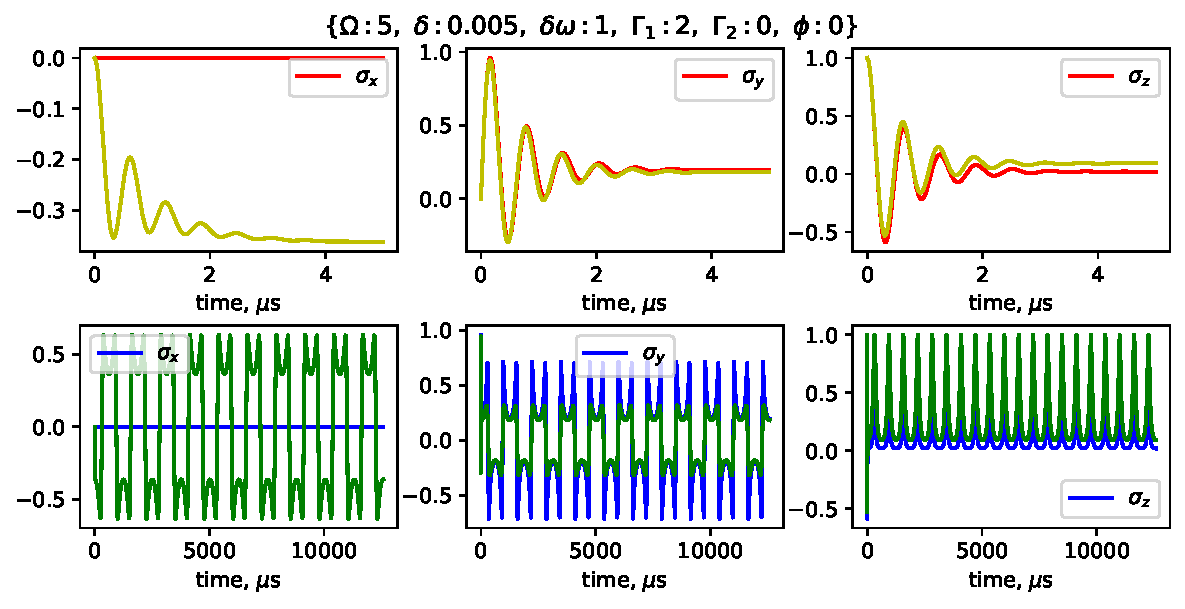
\includegraphics[width=0.9\textwidth]{2drives_num.pdf}
\caption[Численное решение уравнений Блоха для двухуровневой системы для случая бихроматической накачки]{Средние значения атомных операторов в зависимости от времени, полученные при помощи численного решения уравнений \eqref{eq: bloch_bich}. Численные значения параметров (МГц) указаны в заголовке рисунка. Верхний ряд графиков показывает динамику кубита до затухания, а нижний ряд --- дрейф стационарного состояния за счет отстройки. На каждом из графиков пара кривых соотвествует значениям $\Delta\omega=0$~МГц (красная и синяя линии) и $\Delta\omega=1$~МГц (желтая и зеленая линии).}
\end{figure}
\begin{figure}[t]\label{fig: bloch_num_bich}
	\centering
	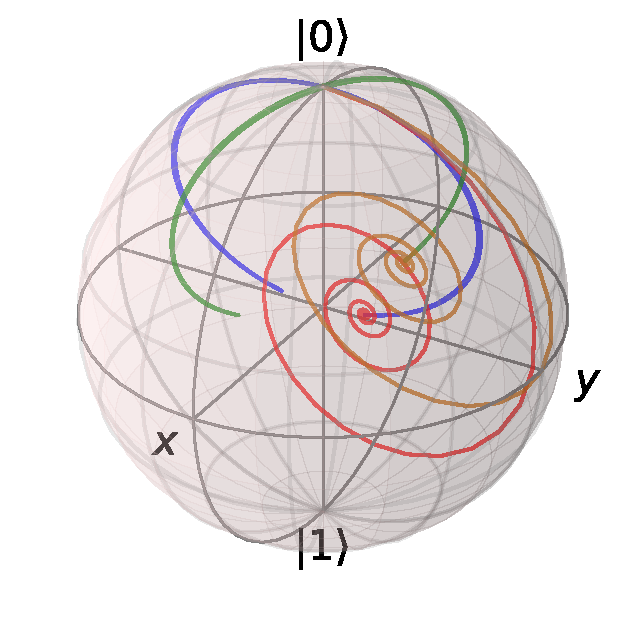
\includegraphics[width=0.6\textwidth]{bloch_2drives_num.pdf}
	\caption[Представление численное решение уравнений Блоха для случая бихроматической накачки на сфере Блоха]{Отображение представленных на Рис.~\ref{fig: num_bich} кривых на сфере Блоха. Дрейф стационарного состояния представляет собой движение по некоторой плоской кривой, поворот которой меняется в зависимости от глобальной отстройки $\Delta\omega$.}
\end{figure}
Для симуляции динамики кубита можно использовать пакет \verb|QuTiP|, реализующий широкий спектр расчетов с квантовыми объектами на базе вычислительных библиотек языка программирования \verb|Python|. Основное квантовое уравнение решается при помощи функции \verb|mesolve|, которая также может рассчитать зависимость среднего значения указанных в аргументах операторов от времени. Как мы отмечали ранее, уравнения Блоха для случая бихроматической накачки имеют вид:
\begin{equation} \label{eq: bloch_bich}
	\dot{\boldsymbol{\sigma}} =\mathbf{M}_b\cdot \boldsymbol{\sigma} + \mathbf{B},
\end{equation} где $\mathbf{B} = [0,\quad 0, \quad-\Gamma_1]^{T}$, a матрица $\mathbf{M}_b$ имеет вид:
\begin{equation}\label{eq: bloch_bich}
	\mathbf{M}_b = \left[\begin{matrix}- {\Gamma}_{2}  & 0 & - 2 \Omega \cos{\left(\delta\omega t + \phi \right)}\\0 & - \Gamma_{2} & - 2 i \Omega \cos{\left(\delta\omega t + \phi \right)}\\\Omega \cos{\left(\delta\omega t + \phi \right)} & - i \Omega \cos{\left(\delta\omega t + \phi \right)} & - \Gamma_1\end{matrix}\right]
\end{equation}
Численное решение этих уравнений приведено на Рис. \ref{fig: num_bich}, для параметров, соотвествующих приближению слабо отстроенных драйвов. Более информативно анализировать результат, построив графики на сфере Блоха, см. Рис.~\ref{fig: bloch_num_bich}. Динамика кубита качественно не отличается от случая однотоновой резонансной накачки, но появляется дрейф стационарного состояния за счет медленно меняющейся фазы. Если мы увеличим отстройку частот накачки, то динамика становится более насыщенной, и вместо стационарного состояния решение более похоже на незатухающую динамику с некоторыми метастабильными точками, возле которых состояние задерживается дольше. 
\begin{figure}[t]\label{fig: bloch_num_bich2}
	\centering
	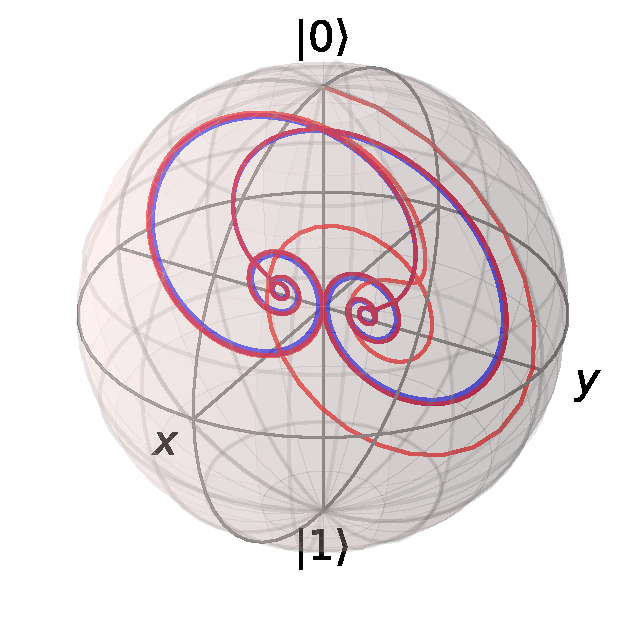
\includegraphics[width=0.6\textwidth]{bloch_2drives_num2.pdf}
	\caption[Численное решение уравнений Блоха для случая бихроматической накачки на сфере Блоха, для случая $\delta\omega \approx \Gamma_1$]{Решение уравнений Блоха при $\delta\omega=0.7$~МГц, остальные параметры совпадают со значениями для кривых на Рис.~\ref{fig: num_bich}. Красная линия отражает начальный этап динамики, синяя --- демонстрирует динамику после стабилизации.}
\end{figure}
В разделе \ref{sec: anal_sol} показано, что волновое смешение можно получить из разложения в спектр поля, которое излучается в слабо менябщемся  квазистационарном состоянии с переменной фазой. Имея численное решение, мы можем получить аналогичный результат при взятии численного преобразования Фурье. Результат изображен на Рис.~\ref{fig: mix_fft} и количественно совпадает с экспериментальными данными на Рис.~\ref{fig: CWM}с). Аналогично можно расчитать, например, зависимость боковых компонент от $\Omega$, и также получить хорошее количественное  совпадение с экспериментом, см. Рис. \ref{fig: mix_fft_omega}.
\begin{figure}[t]\label{fig: mix_fft}
	\centering
	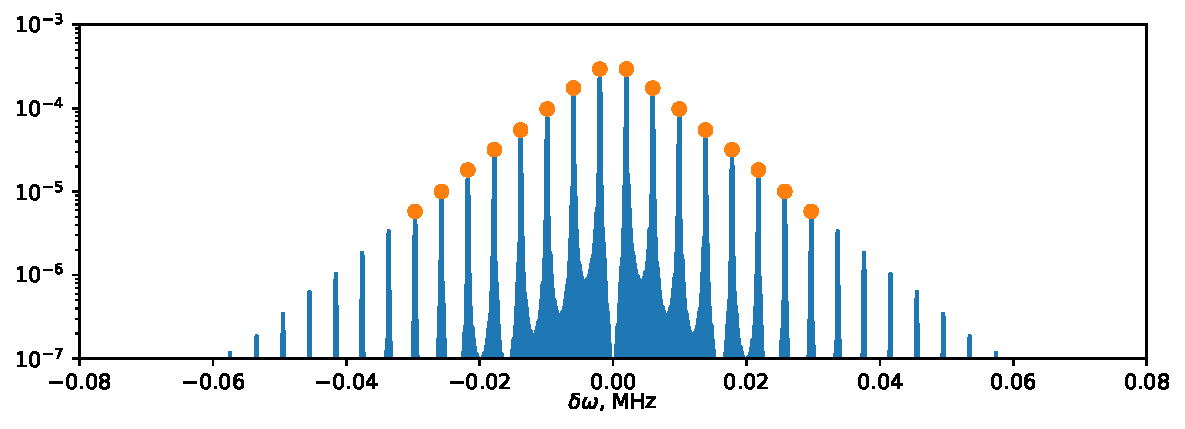
\includegraphics[width=0.99\textwidth]{fft_spec.pdf}
	\caption[Компоненты смешивания волн, полученные как спектр поля, излучаемого в стационарном состоянии]{Компоненты смешивания волн, полученные как спектр поля, излучаемого в стационарном состоянии. Параметры решения приведены в заголовке к Рис.~\ref{fig: num_bich}.}
\end{figure}
\begin{figure}[t]\label{fig: mix_fft_omega}
	\centering
	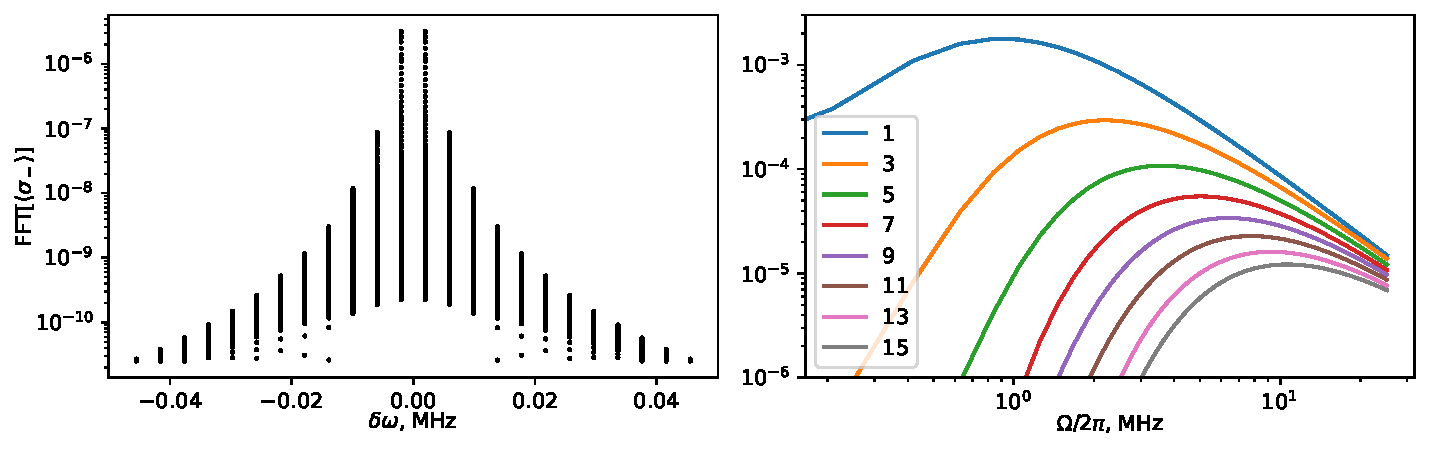
\includegraphics[width=0.99\textwidth]{mixing_Omega.pdf}
	\caption[Зависимость дополнительных компонент от Раби частоты двух управляющих сигналов]{Зависимость дополнительных компонент от Раби частоты $\Omega = $ двух управляющих сигналов, полученная как Фурье-спектр численного решения уравнений Блоха. Слева: значения компонент поля при всех исследуемых $\Omega$. Справа: зависимость компонент различных порядков от $\Omega$.  Параметры решения приведены в заголовке к Рис.~\ref{fig: num_bich}.}
\end{figure}

В данном разделе мы показали, что численное решение уравнений Блоха хорошо описывает эксперимент по смешению бихроматической накачки на кубите. В дальнейшем мы используем этот факт для интерпретации измерений спектра когерентного рассеяния при импульсной бихроматической накачке, когда получение точного аналитического решения более затруднительно.
 
\section{Расщепление Аутлера-Таунса для боковых компонент}
Еще один любопытный эффект, наблюдаемый при измерении когерентной части рассеиваемого кубитом поля --- расщепление интенсивности компонент при изменении глобальной отстройки $\Delta\omega$ между частотой кубита и центральной частотой накачки. Матрица $\mathbf{M}_b,$ задающая уравнения Блоха вида \eqref{eq: bloch_bich}, имеет вид:
$$
\mathbf{M}_b = \left[\begin{matrix}- \Gamma_2 & i \Delta\omega & - 2 \Omega \cos{\left(\delta\omega t + \phi \right)}\\i \Delta\omega & - \Gamma_{2} & - 2 i \Omega \cos{\left(\delta\omega t + \phi \right)}\\\Omega \cos{\left(\delta\omega t + \phi \right)} & - i \Omega \cos{\left(\delta\omega t + \phi \right)} & - \Gamma_1\end{matrix}\right],
$$
\begin{figure}[th]\label{fig: autler-townes like}
	\centering
	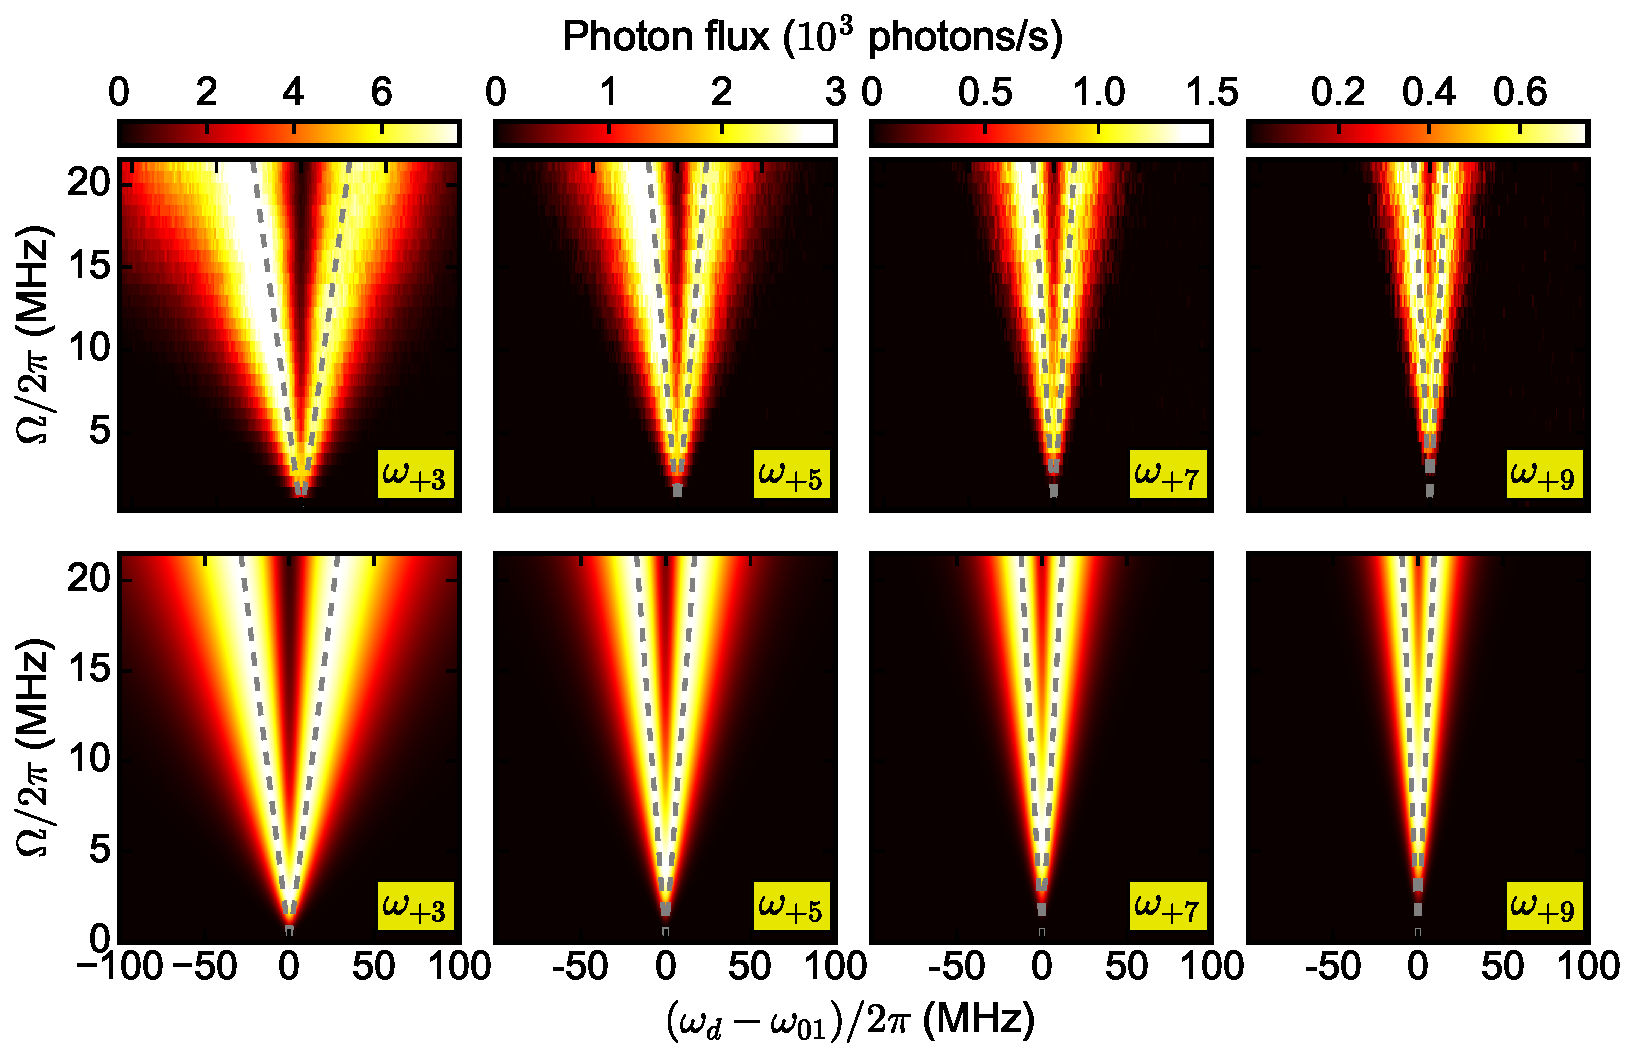
\includegraphics[width=0.95\textwidth]{Fig4_PRA_proofs2.pdf}
	\caption[Расщепление Аутлера-Таунса боковых компонент эластичной части рассеянного на кубите сигнала.]{Расщепление Аутлера-Таунса, наблюдаемое при измерении компонент различного порядка в эластичной части рассеянного на кубите сигнала в зависимости от $\Delta\omega$ и $\Omega$. Верхний ряд графиков представляет измеренные значения $\Omega_{\pm(2p+1)}^{\text{sc}}$, пересчитанные в единицы потока фотонов при помощи выражения \eqref{eq: av_photons}. Нижние панели представляют собой результаты аналитических расчетов согласно \eqref{intensities}. Серые пунктирные линии --- направляющие, соответствующие $\delta\omega = \pm 4\Omega/(2p+1)$. }
\end{figure}
а значение компонент $\Omega_{\pm(2p+1)}^{\text{sc}}$ все так же описывается уравнением \eqref{intensities}. Для измерения зависимостей $\Omega_{\pm(2p+1)}^{\text{sc}}(\Delta\omega)$ не требуется дополнительных технических усложнений: достаточно лишь учесть, что все частоты $\omega_{\pm(2p+1)}$ смещаются также на величину $\Delta\omega$, тогда как частота кубита остается на месте. Результаты измерения этих зависимостей и их сравнения с аналитическими значениями приведены на Рис.~\ref{fig: autler-townes like}. Видно, что с увеличением частоты Раби в эластичной компоненте каждого порядка возникает два расходящихся максимума, расстояние между которыми зависит от порядка спектральной компоненты и хорошо определяется как 
\begin{equation}\label{ATS-like}
	2\Delta\omega = 8\Omega/(2p+1). 
\end{equation}

Полученное расщепление напоминает по своей структуре расмотренный в разделе \ref{AT} эффект Аутлера-Таунса, где расщепление пиков в прохождении резонансного пробного сигнала малой амплитуды является следствием сильной накачки одного из переходов в трехуровневой системе. Однако, имеется ряд существенных различий: система является двухуровневой и мы не прикладываем дополнительный пробный сигнал. Можно предположить, что сильная бихроматическая накачка в сочетании с ненулевой отстройкой создает сложную систему одетых состояний, и переходы между этими состояниями вызывают наблюдаемые картины интенсивностей боковых компонент. Однако, детальный аналитический расчет когеретных компонент с иcпользованием одетых уровней может быть достаточно сложен и до сих пор не встречался в литературе: например, в работе \cite{Ficek_resonance} уравнения решаются численно, но не ставится задача нахождения аналитического решения. Поэтому количественно точное описание расщеплений при помощи системы одетых уровней, бесспорно, являясь крайне интересной физической задачей, тем не менее, выходит за рамки представляемой работы.
\section{Волновое смешение и фотонная статистика в волноводе}
\label{sec: mix_stat}
Как было указано в разделе \ref{sec: maxbloch_num}, волновое смешение может быть использовано в качестве инструмента изучения фотонной статистики в некоторой волноводной моде. В микроволновом диапазоне частот это приобретает особенное практическое значение ввиду отсутствия эффективных детекторов фотонов, и как следствие, техническими сложностями при измерении корреляционной функции поля второго порядка $G^{(2)}(t, \tau)$, которая является общепризнанным стандартным измерением, позволяющим установить квантовость (в частности, однофотонность) распространяющегося поля) и даже выполнить полную томографию поля \cite{Eichler_tomo, EichlerTomography}. Мы можем проиллюстрировать возможность исследования фотонной статистики, опираясь на полученные в данном разделе результаты.

Для иллюстрации возможности восстановления статистики подсчитаем среднее число фотонов в интересующей нас моде, пролетающее мимо кубита на характерном времени $\tau\sim\Gamma_2^{-1}$). Мы выбираем масштаб, отвечающий времени когеретности кубита, поскольку характеризуем именно эластичное рассеяние, для которого важен тот факт, что состояние кубита не потеряло информацию о фазе. Поэтому среднее число фотонов равно $\braket{N} = P(\hbar\omega\Gamma_2)^{-1}$. Мощность излучения в линии можно выразить через амплитуду раби $\Omega$: $P = (\hbar\Omega/\mu)^2/(2Z_0)$. Комбинируя эти выражения с \eqref{eq: G1}, получаем:
\begin{equation} \label{eq: av_photons}
	\braket{N} = \frac{\Omega^2}{\Gamma_1\Gamma_2}.
\end{equation}
Для простоты рассмотрим предел слабой накачки: $\Omega_{\pm} \gg \Gamma_1.$ В этом приближении легко показать, что:
$\theta \approx (\Omega_+\Omega_-)/\Gamma_2^2, \Lambda \approx (2\Omega_+\Omega_-)/{\Gamma_2}
$. При подстановке в \eqref{intensities} получаем:
\begin{equation}\label{eq: 2p+1_approx}
	\Omega_{\pm(2p+1)}^{sc} =\frac{(-1)^{p+1}}{2^{p}}\Gamma_2^{-2p-1}\Gamma_1\Omega_+^{p+1}\Omega_-^p,
\end{equation}
В результате, амплитуда боковой компоненты зависит от степеней апмлитуд исходных полей, показатели которых соответствуют порядку нелинейности. Поэтому и средние числа фотонов подчиняются схожему соотношению:
\begin{equation}\label{eq: N_2p+1}
	\braket{N_{2p+1}} = \braket{N_-}^p\braket{N_+}^{p+1}
\end{equation}
Это полуклассическое рассуждение наводит нас на мысль о том, что среднее число фотонов может не только зависеть от средних $\braket{N_+},\!\braket{N_-}$, но и содержать в себе более подробную информацию о фотонной статистике. Естественно, это предположение невозможно подтвердить для пуассоновских распределений фотонов, для которых первый момент определяет все последующие. Однако, многофотонная природа процессов волнового смешения является сильным аргуменом в пользу того, что интенсивности вновь появляющихся в результате волнового смешения пиков должны быть чувствительны к индивидуальным амплитудам вероятности фоковских состояний в исходных модах $\omega_\pm$ или к каким-либо комбинациям этих амплитуд. Переходя к квантовомеханическому описанию поля, выражение в правой части \eqref{eq: N_2p+1} можно получить также как среднее значение оператора $(a_+a_-^\dag)^pa^+$ на когерентных состояний в двух модах $\ket{\alpha_+, \alpha_-}$ На основе эксперимента с классической накачкой доказать его справедливость невозможно, однако, весьма похожий эффект теоретически рассматривался в работах \cite{WallsMilburn_PRD,PhysRevA.28.2646}. В этих работах изучались различные способы измерения интересующего исследователя квантового объекта, а именно --- гармонического осциллятора с полем $\hat{a}$. В качестве измерителя выступает другой осциллятор $\hat{b}$, испытывающий значительное воздействие со стороны окружения. Считается, что объект взаимодействует с измерителем таким образом, что гамильтониан этого взаимодействия имеет вид:
\begin{equation}
	H_{m-o} = \frac{\hbar}{2}a^\dag a(\Omega b + \Omega^* b^\dag),
\end{equation}
и как утверждается, может быть реализован через волновое смешение на нелинейной восприимчивости третьего порядка. В свою очередь, измеритель отдает свою энергию окружению, состоящему из большого числа осцилляторов:
\begin{equation}
	H_{B-m} = \sum_i^{}\kappa_i\left(B_ib^\dag +B^\dag_i b\right).
\end{equation}
В работе \cite{WallsMilburn_PRD} показано, что в этом случае результирующее состояние системы из двух осцилляторов позволяет осуществить неразрушающее измерение изучаемого объекта в фоковском базисе, при этом стабильный базис измерителя состоит из когерентных состояний и измерение может быть рассмотрено в классическом пределе. Система при этом считается бесконечно долгоживущей, так как нас интересует лишь процесс измерения. Говоря точнее, если задано начальное состояние системы <<объект-измеритель>>:
\begin{equation}
	\rho(0) = \sum_{n,m}^{}\rho_{n,m}(\ket{n}\bra{m})_o\otimes(\ket{0}\bra{0})_m,
\end{equation}
то после затухания когерентности в измерителе состояние стремится к:
\begin{equation}
	\lim_{t \to \infty}\rho(t) = \sum_n^{}\rho_{nn} (\ket{n}\bra{n})_m \otimes
	(\ket{\alpha_n}\bra{\alpha_n})_o,
\end{equation}
где $\alpha_n = \Omega n (1-e^{\gamma t/2})/\gamma$, а $\gamma$ --- скорость релаксации измерителя в окружение. Таким образом, если спроецировать измеритель на когерентное состояние, то объект окажется в фоковском состоянии. Также показано, что если накапливать отсчеты детектора фотонов, проецирующего состояние измерителя, то полное число отсчетов при условии быстрого измерения и сильной связи с полем $\Omega$ пропорционально $\braket{a^\dag a}^2$. Эти результаты подтверждают выдвинутые предположения о применимости наблюдаемого эффекта для измерений числа фотонов в распространяющихся мимо кубита модах. 

Подводя итоги вышесказанному, продемонстрирован фундаментальный эффект волнового смешения стационарных когерентных состояний на одном двухуровневом рассеивателе, сильно связанном с одномерной линией передачи. Мы получили аналитическое выражение для амплитуд смешанных состояний и показали ряд других физических эффектов, например, подобное Аутлеру-Таунсу расщепление боковых пиков в зависимости от числа рассеянных фотонов. Боковые пики являются результатом процессов многофотонного рассеяния, а их амплитуды определяются распределением фотонов в когерентных состояниях. Интересным будущим применением будет визуализация статистики неклассических когерентных состояний. Использование волнового смешения сигналов на кубите для восстановления фотонной статистики этих сигналов может стать весьма перспективным применением полученных в данной работе результатов. Однако, это утверждение требует дополнительной экспериментальной проверки. В следующем разделе мы обратимся к импульсному драйву кубита в различных исполнениях и покажем, что спектр рассеяния импульсной накачки крайне чувствителен к разрешенным и запрещенным многофотонным процессам рассеяния, и модифицируется в соотвествии с числом фотонов, доступных для реализации того или иного процесса. 


 




